% !TeX spellcheck = en_US

\chapter{Practical Results}\label{chp:practical_results}

\section{QGIS Plugin}
A QGIS plugin has been created, which allows to process the currently displayed imagery in a corresponding backend server. \autoref{fig:plugin:changes} shows an image of the imagery layer overlayed with the changes generated by the backend. \autoref{fig:plugin:changes_cadastral_layer} shows the same changes on the cadastral data layer and \autoref{fig:plugin:predictions} shows the predictions as returned by the neural network.

\begin{figure}[H]
    \centering
	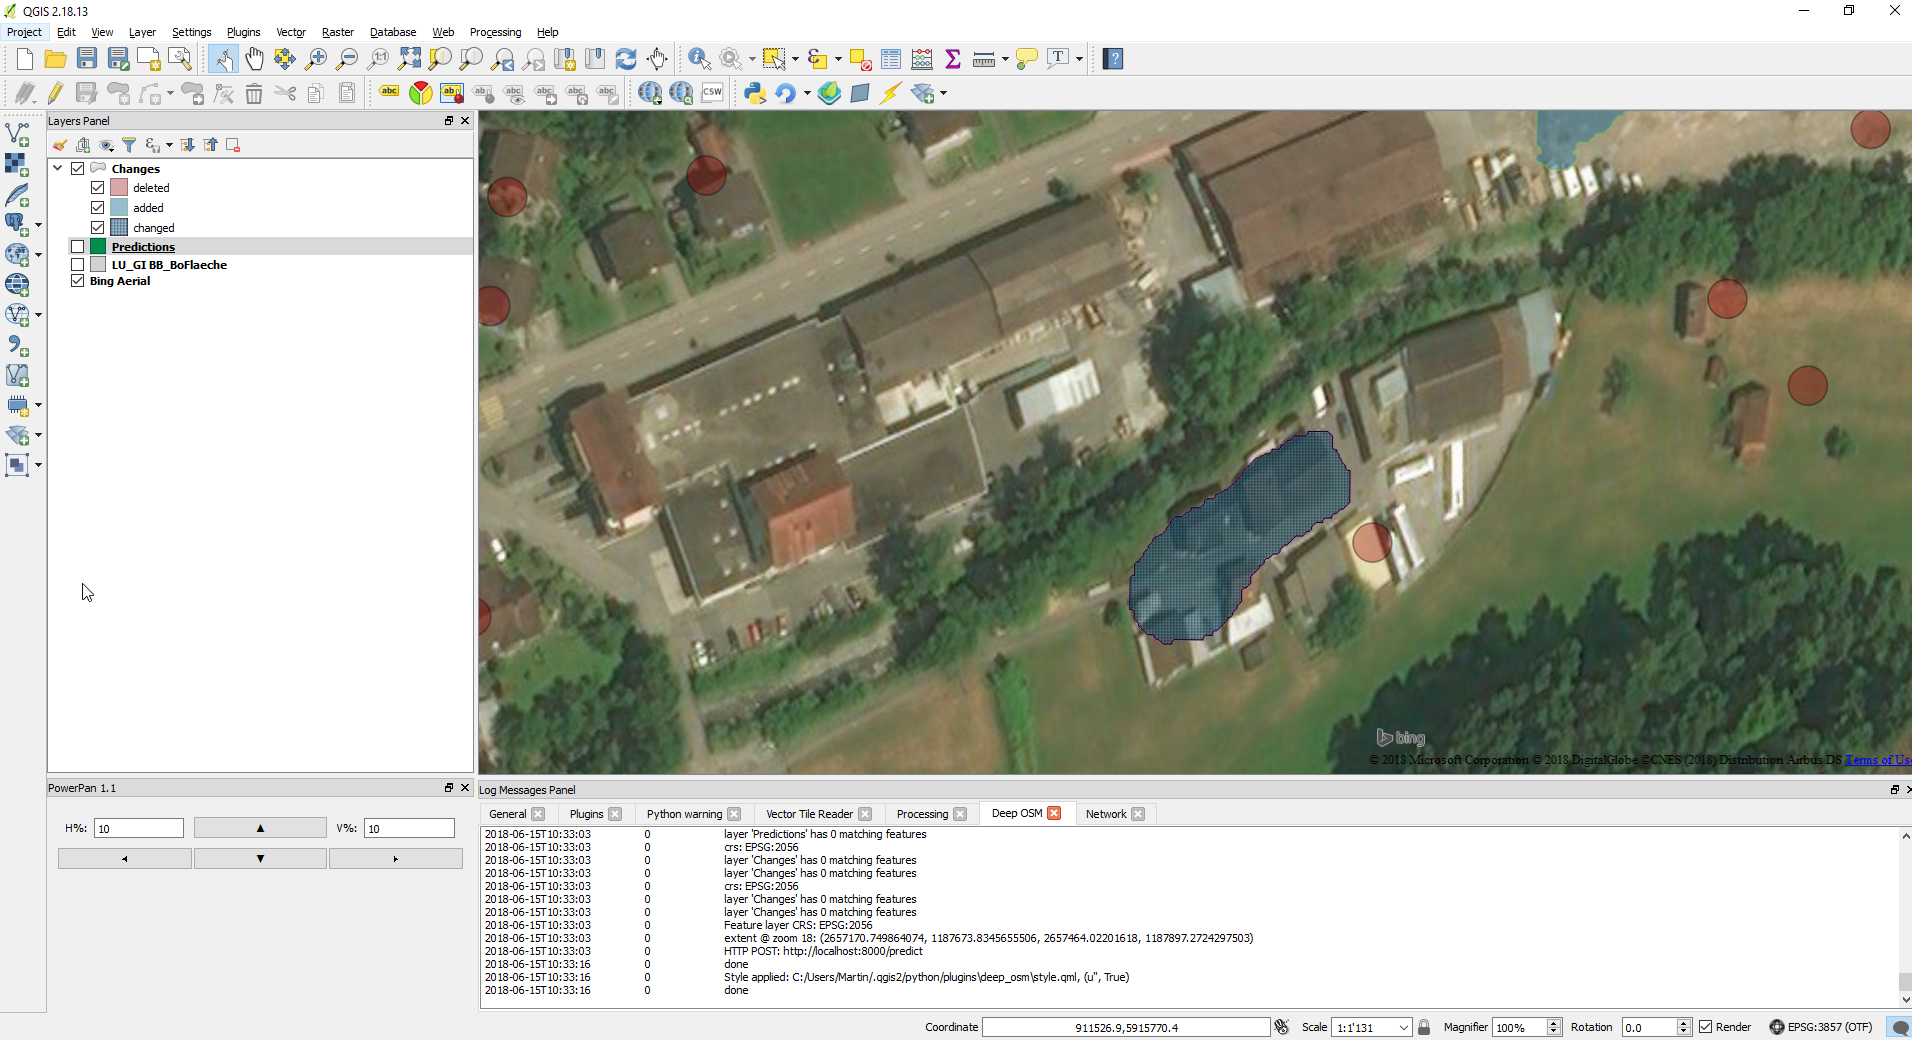
\includegraphics[width=1\linewidth]{chapters/practical_results/images/qgis_changes_aerial.png}
	\caption{Changes in QGIS}
	\label{fig:plugin:changes}
\end{figure}

\begin{figure}[H]
    \centering
	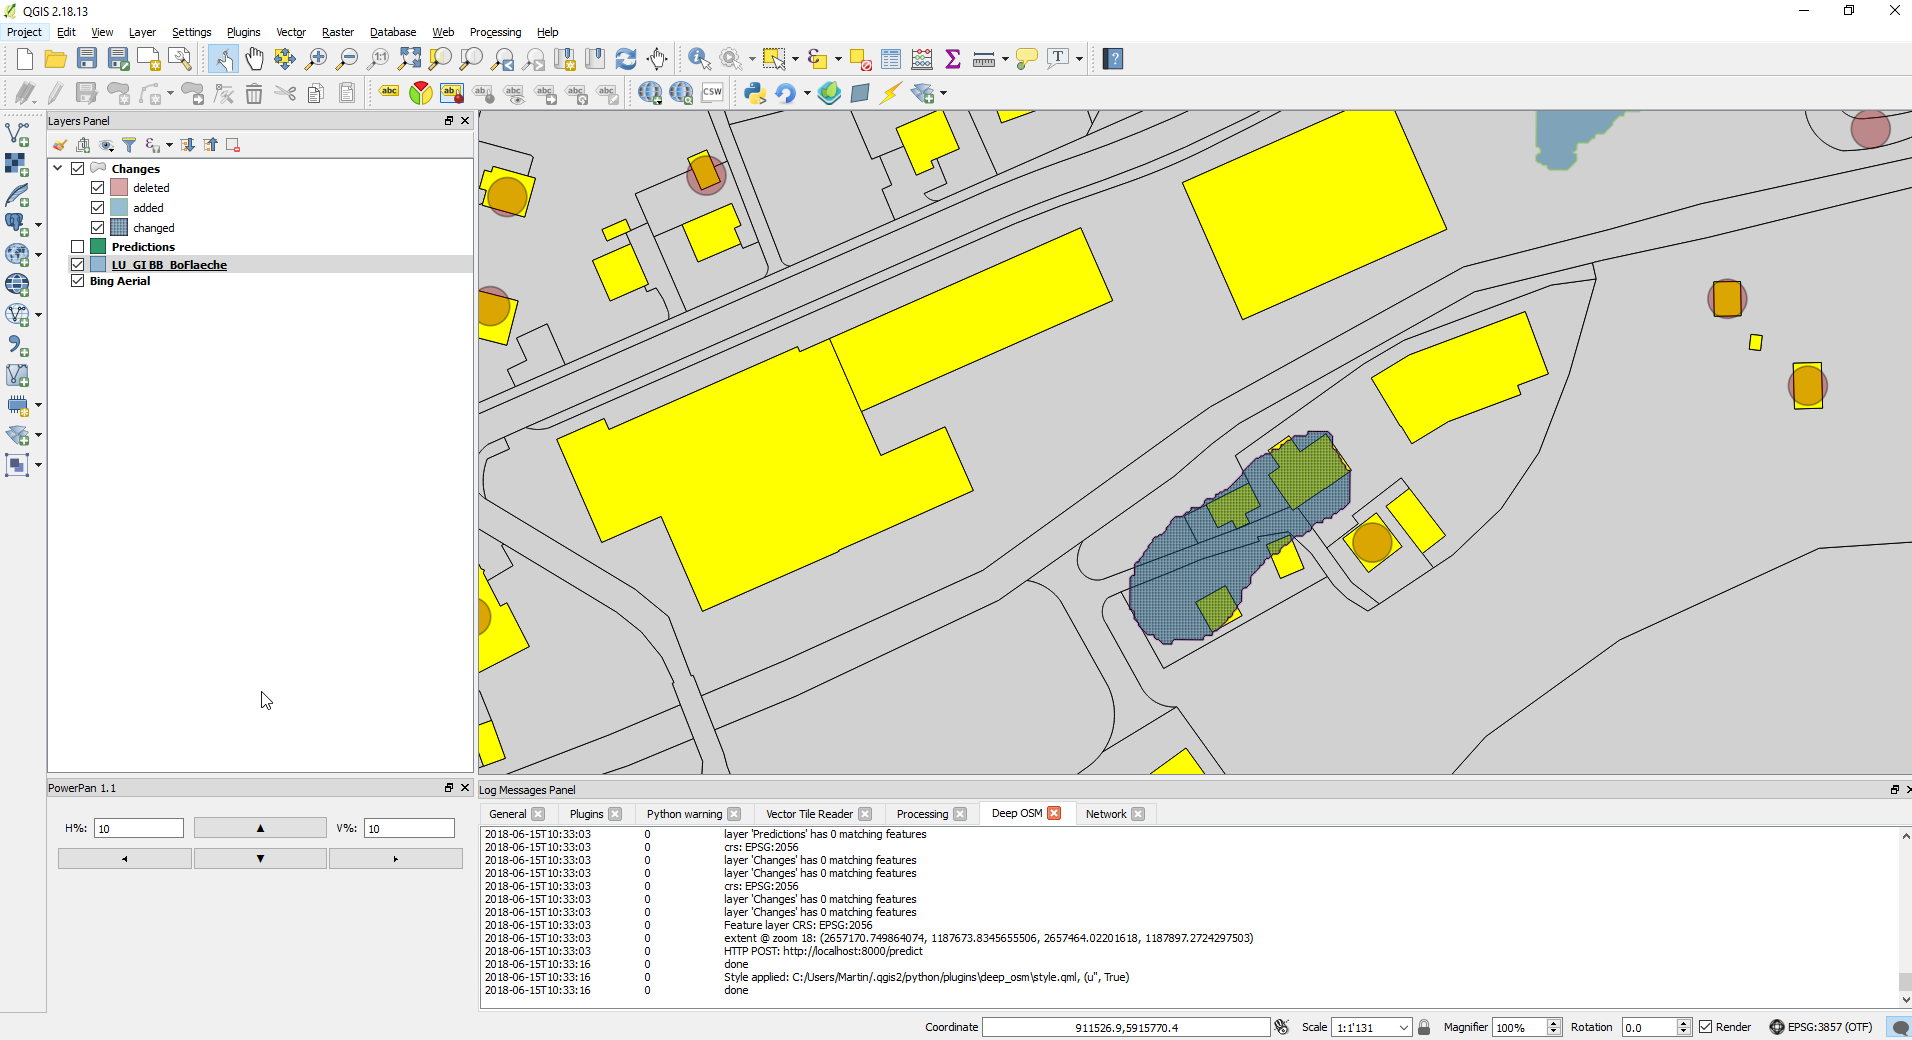
\includegraphics[width=1\linewidth]{chapters/practical_results/images/qgis_changes.png}
	\caption{Changes on cadastral survey data layer}
	\label{fig:plugin:changes_cadastral_layer}
\end{figure}

\begin{figure}[H]
    \centering
	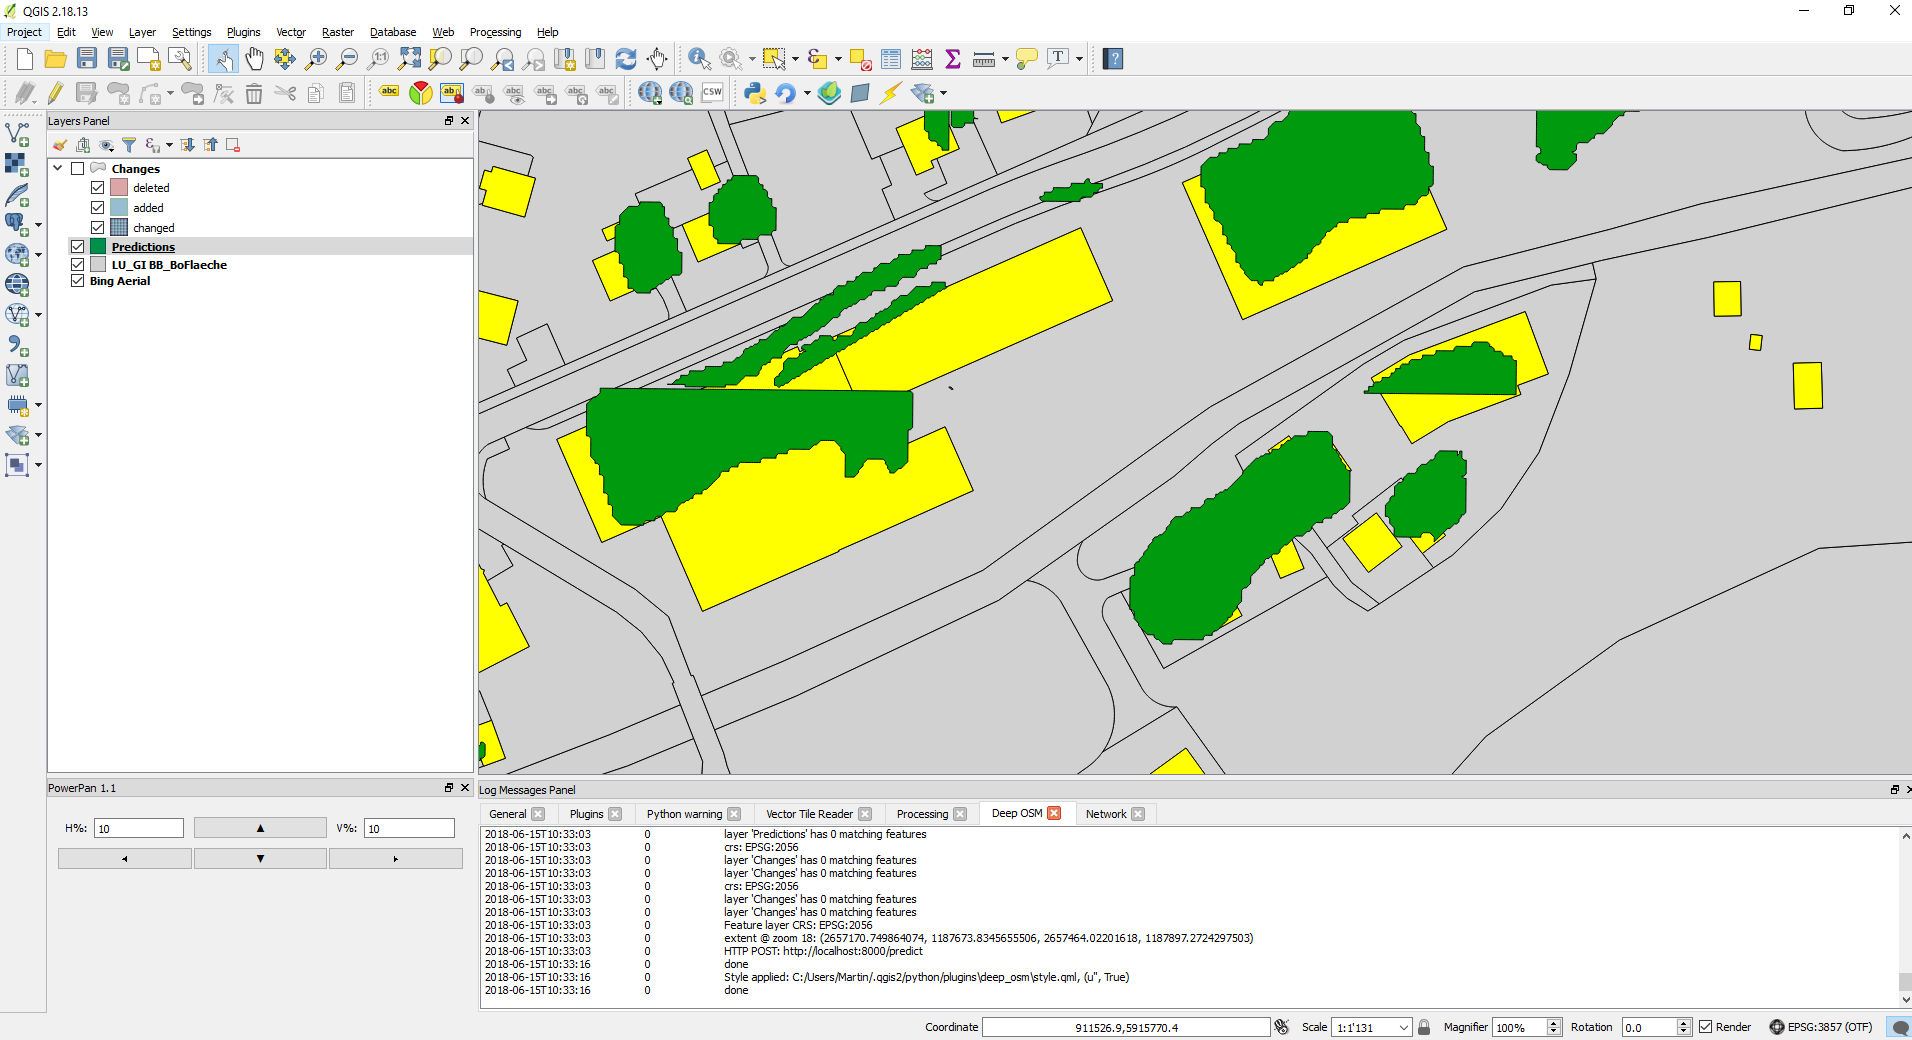
\includegraphics[width=1\linewidth]{chapters/practical_results/images/qgis_predictions.png}
	\caption{Predictions (green) as generated by the neural network}
	\label{fig:plugin:predictions}
\end{figure}

\begin{figure}[H]
    \centering
	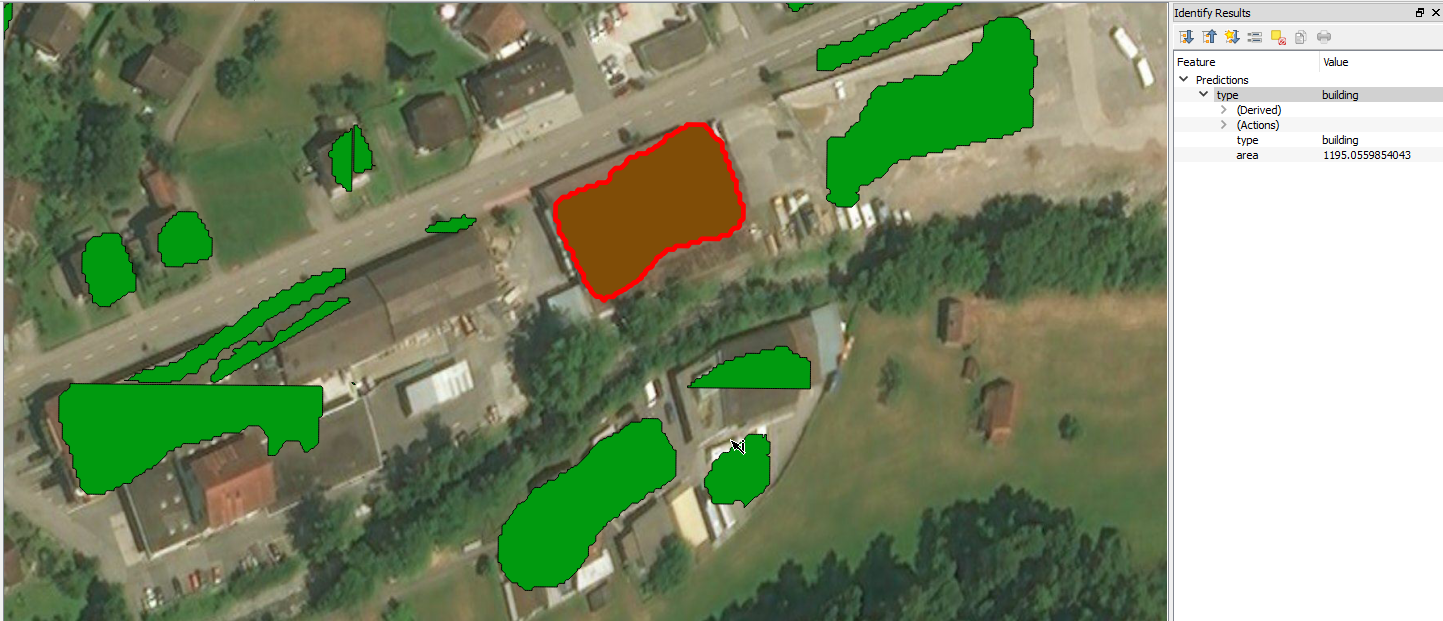
\includegraphics[width=1\linewidth]{chapters/practical_results/images/qgis_prediction_attributes.png}
	\caption{Predictions have attributes showing the predicted class (building in this case)}
	\label{fig:plugin:prediction_attributes}
\end{figure}

\begin{figure}[H]
    \centering
	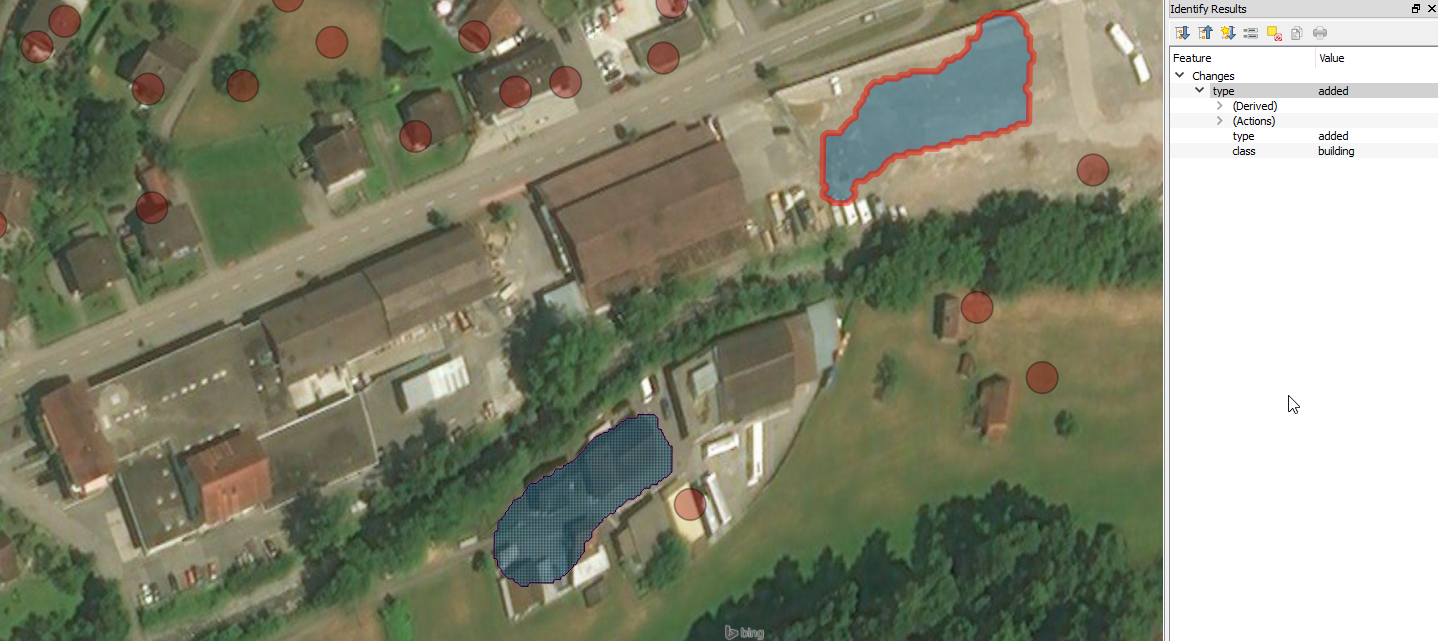
\includegraphics[width=1\linewidth]{chapters/practical_results/images/qgis_changes_attributes.png}
	\caption{Changes have attributes showing the predicted class and the type of change (added, deleted, changed)}
	\label{fig:plugin:change_attributes}
\end{figure}

\subsection{User Scenario}

\subsection{Effizienzsteigerung}

\section{Semantic Segmentation}
The trained network performs best for the building class, which is a result of the imbalanced dataset. The imbalancedness is a result of the 